\section{Star Partition and Mining}
\label{sec:spm_solution}
TRM approach requires to replicate entire
trajectories $O(|\mathbb{T}|)$ times, which is inefficient
in parallelism. To overcome this limitation, we 
propose the \emph{Star Partition and Mining} (SPM) method.
In SPM, we design a graph model, named \emph{connection graph}, to capture 
the co-moving behavior among objects. In such a way, 
given an object $u$, all the objects potentially
co-moved with $u$ are captured in $u$'s neighborhood, which
forms a \emph{star} structure in graph terms. SPM utilizes
such structures to partition objects and then adapts an Apriori 
algorithm to discover true GCMPs from each partition.

The flow of SPM method is presented in Figure~\ref{fig:star_partition}.
SPM utilizes the same preprocessing as TRM, thus the flow starts
from clusters in each snapshot. Conceptually, the clusters 
in each snapshot forms a graph as shown in Figure~\ref{fig:star_partition} (a).
In the map phase of \emph{SPM}, a vertex together with its neighborhood 
vertexes form a star. Every star is indeed an independent partition.
Then, stars are shuffled to reducers. As in
Figure~\ref{fig:star_partition} (c), Apriori mining algorithm is adapted
to mine the GCMP patterns. The overview implementation of SPM is shown 
in Algorithm~\ref{algo:spm_overview}.

%The overview of the SPM method is presented in 
%Algorithm~\ref{algo:spm_overview}. As shown, SPM takes three phases. 
%In the map phase, objects from the same cluster form object-object pairs. 
%The object-object pairs are then paired up with the timestamp of 
%the snapshot to form a triplet(lines~\ref{code:spm-map-start}-\ref{code:spm-map-end}). 
%In the partition phase, triplets with the same leading object form a \emph{star} which will be explained shortly 
%(lines~\ref{code:spm-shuffle-start}-\ref{code:spm-shuffle-end}).
%Lastly in the reduce phase, patterns are mined from each star structure (lines~\ref{code:spm-reduce-start}-\ref{code:spm-reduce-end}).

\begin{algorithm}
\caption{Star Partition and Mining}
\label{algo:spm_overview}
\begin{algorithmic}[1]
\Require list of $\langle t, S_t \rangle$ pairs
\State {---Map phase---}
\label{code:spm-map-start}
\ForAll{$C \in S_t$}
	\ForAll {$(o_1 ,o_2) \in C \times C$}
		\If{$o_1 < o_2$}  \label{code:spm-edge-direct}
			\State emit a $\langle o_1, o_2, \{t\}\rangle$ triplet
		\EndIf
	\EndFor
\EndFor
\label{code:spm-map-end}

\State {---Partition and Shuffle phase---}
\label{code:spm-shuffle-start}
\ForAll{$\langle o_1, o_2, \{t\}\rangle$ triplets} 
	\State group-by $o_1$, emit $\langle o_1, Sr_{o_1} \rangle$ 
	%\State group-by $o_2$, emit $\langle o_2, Sr_{o_2} \rangle$
\EndFor
\label{code:spm-shuffle-end}

\State {---Reduce phase---}
\label{code:spm-reduce-start}
\ForAll{$\langle o, Sr_{o} \rangle$}
\State Apriori($Sr_o$)
\EndFor
\label{code:spm-reduce-end}

\end{algorithmic}
\end{algorithm}

\subsection{Star Partition}
The intuition of the star partition is that, if two objects are part 
of the same pattern, they must belong to the same cluster at 
those snapshots. Therefore, we may link objects that belong to 
the same cluster to form the \emph{connection graph}. Objects that are
not connected surely fail to form a pattern. We may then
partition the connection graph based on vertex connectivity
such that mining GCMPs can be done in parallel. 
We formally define the \emph{connection graph} as follows:
\begin{definition}[Connection Graph]
A connection graph is an undirected graph $G=(V:E)$, where 
each $v \in V$ represents an object. An edge $e(s,t)= ET \in E$ 
contains the timestamp sequence at which $s,t$ are in the same cluster,
i.e., $\forall t \in ET, C_t(s) = C_t(t)$. 
\end{definition}

In graph theory, a \emph{star} of a vertex $u$ is the
the set of neighborhood vertexes of $u$. To utilize \emph{star}
partition, since a vertex may appear in multiple stars, 
some replications of vertexes are required. In order to avoid replication 
of edges, we use the \emph{directed star} as follows:

\begin{definition}[Directed Star]
Assign each vertex in $G$ an ID, a direct star of a vertex $s$, denoted as $Sr_s$, 
is the set of incidental edges on $s$
such that $\forall e(s,t) \in Sr_s$, $s < t$. We name $s$
as the \emph{central vertex} of $Sr_s$.
\end{definition}

By leveraging the \emph{directed star}, we avoids replicating the edges. 
A \emph{Connection graph} and \emph{star} examples are 
shown in Figure~\ref{fig:star_partition} (a) and (b). In (a), a connection graph is formed
based on the example in Figure~\ref{fig:related_work}.
In (b), 5 stars are presented. It can be figured out that by leveraging directed star, 
no edges are replicated. In implementation,
as show in Algorithm~\ref{algo:spm_overview} line~\ref{code:spm-edge-direct}, the
comparison between vertices/objects are based on the vertex/object IDs.

\begin{figure*}[t]
\centering
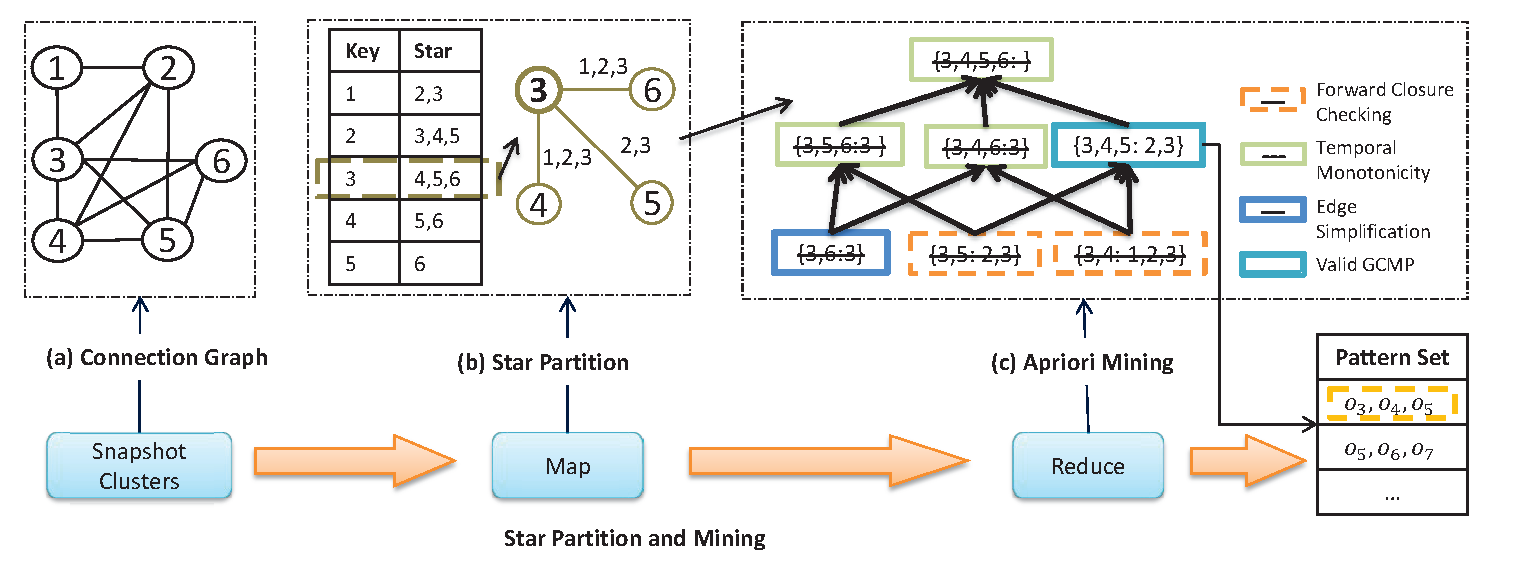
\includegraphics[width=0.9\textwidth]{spm.eps}
\caption{Star partition and mining. (a) Conceptual connection graph from Figure 1.(b) Five star partitions are generated
(c) Apriori Mining with various pruning techniques.}
\label{fig:star_partition}
\end{figure*}

%After computing the star, each partition is applied with a reduce task. 
%Indeed, a star $Sr_s$ can be viewed as a subset of original trajectories. 
%This is done by treating each vertex in $Sr_s$ as an object. 
%The time sequence of $s$ is the union of all edges in $Sr_s$. 
%And the time sequence of $v \neq s$ is the edge $(s,v)$. Therefore, we
%are able to mine stars from the similar trajectory concepts.

\subsection{Apriori Mining}
To systematically discover valid patterns in each star, 
we design the \emph{Apriori Mining} algorithm. 
To describe the  algorithm, we call a candidate pattern $R$-pattern 
if the size of its object set is $R$.  Therefore, each edge
in the star is effectively a $2$-pattern. The intuition of Apriori mining
is the observation that $(R+1)$-patterns can be generated
from $R$-patterns and $2$ patterns. Thus, we may iteratively 
enumerate pattern candidates with all possible sizes.
In particular, initially, for each $e(s,v)=ET$, pattern $p=(\{s,v\}, ET)$ is formed. 
During each iteration, we generate $(R+1)$-patterns by joining $R$-patterns 
with the $2$-patterns. Technically, the join between $p_1=(O_1:T_1)$ and $p_2=(O_2:T_2)$
generates a new pattern $p_3=(O_1 \cup O_2:T_1 \cap T_2)$. Note that in $Sr_s$,
each $R$-pattern contains the object $s$, thus the join only 
grow a $R$-pattern at most to a $(R+1)$-pattern.
Our mining algorithm stops where no further patterns are generated. 
The algorithm is illustrated as in Algorithm~\ref{algo:apriori_mining}.

\begin{algorithm}
\caption{Apriori Mining}
\label{algo:apriori_mining}
\begin{algorithmic}[1]
\Require{$Sr_s$}
\State { Lv $\gets \{\}$,Ground $\gets \{\}$, Output $\gets \{\}$}
\ForAll{$e(s,t) = T \in Sr_s$}
\State Ground.add($\langle \{s,t\}, T \rangle$);
\State Lv $\gets$ Ground;
\EndFor
\While{true}
	\If{Lv is not empty} 
		\State{LvCand $\gets \{\}$ }
		\ForAll{$cand_v \in Lv$}
			\ForAll{$cand \in $Ground}
				\State $p \gets cand_v$ join $cand$
				\If{$p.T$ is a candidate sequence} 
					\State LvCand.add($p$)
				\EndIf
			\EndFor
		\EndFor
		\If{$Lv$ is a pattern}
			\State{Output.add($Lv$)}
			\State{break}			 
		\EndIf
		\State {Lv $\gets$ LvCand}
	\Else
		\State{break}
	\EndIf
\EndWhile
\State output.addAll($Lv$)
\State \Return output
\end{algorithmic}
\end{algorithm}
 
An illustration of Algorithm~\ref{algo:apriori_mining} is shown in Figure~\ref{fig:star_partition} (c).
As shown, the star $Sr_3=\{3,4,5,6\}$ initially generate three $2$-candidates. At every iteration, 
higher level candidates are generated by joining lower level candidates. When no more candidates 
can be generated, the algorithm stops by outputting the valid patterns.

It is notable that, in star partition, original data is 
replicated for $O(|\mathbb{O}|)$ times as each object may 
be sent to $O(|\mathbb{O}|)$ stars. Since in reality, $|\mathbb{T}| \gg |\mathbb{O}|$, 
the star partition is more scalable than the temporal replication.
In later sections, we will describe several engineering level optimization to further reduce the amount of replicated data.
%It is notable that Algorithm~\ref{algo:apriori_mining} takes exponential
%time to mine GCMP. There are two major factors dragging 
%down the performance. First, the size of $Sr_s$ affects the initial 
%size of $2$-patterns. Second, the candidates generated in each 
%level affects the join performance. In later
%sections, we exploit some properties of GCMP to reduce the two factors.

\subsection{Analysis of SPM}
The analysis of SPM contains two parts. We first prove the correctness
of SPM. Then, we analyze the work load distribution of the star sizes.

\subsubsection{Correctness}
Although star partition is performed based on the connection graph, 
each star is indeed a projection of original trajectories.
To see this, each vertex can be viewed as an object. 
The timestamps of center vertex $s$ is the union of all the 
edges in $Sr_s$. The timestamps of vertex $v \neq s$ is the 
edge $e(s,v)$. Therefore, stars can be viewed as a trajectory
database, where GCMP can be similarly defined. Using the same 
notions as Definition 4, we state the correctness
of star partition as follows:

\begin{theorem}[Soundness and Completeness of Star Partition]
Star partition is sound and complete.
\end{theorem}

\begin{proof}
For the soundness,
if $P$ is a valid pattern in $Sr_s$, then at every time $t$, 
$\forall o_1, o_2 \in P.O$, $C_t(o_1) = C_t(o_2)$.
By definition, $P$ is valid in the original trajectories.
For the completeness,
if $P$ is a valid pattern in original trajectories, 
let $s$ be the object with smallest ID in $P.O$. 
Based on the definition of GCMP, $\forall t \in P.T$, $\forall o \in P.O$, $C_t(s) = C_t(o)$.
It follows that all object $o \in P.O$ are in $Sr_s$. 
Furthermore, every timestamp in $P.T$ is included
in $Sr_s$. Therefore, $P$ is a valid pattern in $Sr_s$.
\end{proof}


\subsubsection{Optimal Star Partition}
An important concern in design parallel algorithms is 
the distribution of work loads. Unlike TRM where each partition
contains equal-sized snapshot, the size distribution 
of stars remains SPM unknown. 
Traditionally, the quality of a partition strategy 
is measured based on two aspects: (1) the number of result partition, which
affects the maximum parallelism
(2) the balance of partition sizes, which affects the finishing
time of a job. We notice that, in star partition, the total sizes of 
stars are invariant. Therefore, the quality of a partition strategy
can be formalized as the \emph{skewness}, which is the maximum star size
among all stars. Smaller \emph{skewness} naturally results in more partitions
and less imbalance.


\begin{figure}[h]
\centering
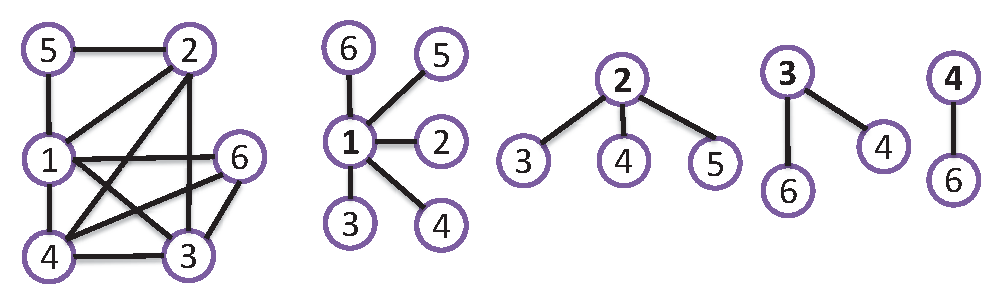
\includegraphics[width=0.4\textwidth]{star-alt.eps}
\caption{An alternative numbering and partitioning of the connection graph in Figure~\ref{fig:star_partition}.}
\label{fig:star-alt}
\end{figure}

Interestingly, we note that the \emph{skewness} of star partition is affected by
the way the vertexes are numbered in the connection graph. For example,
Figure~\ref{fig:star-alt} gives two valid numbering of vertexes 
in the same connection graph, but produces two different set of stars. 
The upper partitioning constructs four stars with the maximum star consisting of 5 edges.
The lower partitioning constructs five stars with the maximum star consisting of 3 edges.
Apparently the upper partitioning is inferior because its \emph{skewness} is 5 while the
lower one's \emph{skewness} is 3.

Ideally we wish to find a numbering scheme of connection graph
that minimize the \emph{skewness}.
To quantify the objective, we design an linear algebra model as follows: Let $G$ denote a connection graph.
Let $\mathbb{A}$ be an arbitrary numbering of vertexes in $G$.
Let $(A:a_{i,j})$ be a boolean assignment matrix wrt. $\mathbb{A}$ (i.e., $a_{i,j}$ indicates whether vertex $j$ is included in $Sr_i$). Let vector $\vec{b}$
be the \textit{one}\footnote{Every element in $\vec{b}$ is $1$} vector. Let $\vec{c} = A\vec{b}$, then
each $c_i \in \vec{c}$ denotes the size of star for vertex $i$.
Therefore, minimizing the \emph{skewness} can be formulated as follows:
\begin{equation}
\mathbb{A}  = \argmin(||A\vec{b}||_\infty) \text{,where } ||A\vec{b}||_\infty = \max_{1\leq j \leq n}(c_j)
\end{equation}

It is challenging to directly optimize the above equation. 
First, suppose there are $n$ vertexes in $G$, enumerating
all possible $\mathbb{A}$s leads to $n!$ combinations. 
Such a high complexity is trivially unpractical. Second,
since $G$ is only conceptual at runtime, 
the load planning cannot be done beforehand. 
Despite these challenges, we observe that there is a 
$O(1)$ time solution which is good enough as stated in the 
following theorem.

\begin{theorem}[Balance of Star Partition]
Let $G$ be a connection graph with $n$ vertexes and the average degree $d$.
Let $\mathbb{A}^*$ be the optimal numbering wrt. Equation 1.
For any numbering, $\mathbb{A}$, with high probability, the 
absolute skewness difference between $\mathbb{A}^*$ and $\mathbb{A}$ is $O(\sqrt{n \log n})$.
That is, it is very likely that 
$||\mathbb{A}\vec{b}||_\infty = ||\mathbb{A}^*\vec{b}||_\infty + O(\sqrt{n \log n})$.
\end{theorem}

\begin{proof}
Let $\mathbb{A}^*$ be the optimal solution wrt Equation 1. Since we have a star
for each object, by the degree-sum formula and pigeon-hole theorem, $||A^*\vec{b}||_\infty \geq d/2$.
Next, let $e_{i,j}$ be an entry in the adjacent matrix of $G$. Note that edges in $G$ are independent. 
Let $d_i$ denote the degree of vertex $i$ in $G$. 
It follows that $E[d_i]=E[\Sigma_{1\leq j \leq n}e_{i,j}]=d$.
Since in the star partition, each edge is assigned to the vertex
with smaller IDs, the connection between $a_{i,j}$ and $e_{i,j}$ can be written as:
\begin{equation*}
a_{i,j} = \begin{cases}
			e_{i,j}, i>j \\
			0, otherwise
		  \end{cases}  
\end{equation*}
There are two observations made on the above equation. First, since $e_{i,j}$s are independent,
$a_{i,j}$s are independent. Second, since $i>j$ and $e_{i,j}$ are independent. 
$E[a_{i,j}] = E[e_{i,j}]E[i>j]= E[e_{i,j}]/2$.

By definition, $c_i = \Sigma_{1\leq j \leq n} a_{i,j}$, 
is a sum of $n$ independent 0-1 variables. Taking expectation on both sides, 
we get: $E[c_i] = E[\Sigma_{1\leq j \leq n} a_{i,j}]=E[\Sigma_{1\leq j \leq n} e_{i,j}]/2 = d/2$. Let $\mu =E[c_i] = d/2$, 
$t = \sqrt{n\log n}$, by Hoeffding's Inequality, the following holds:
\begin{equation*}
\begin{split}
	Pr(c_i \geq \mu + t) 
						&\leq \exp(\frac{-2t^2}{n}) \\
						&= \exp(-2\log n) = n^{-2}
\end{split}
\end{equation*}

The first step is due to the fact that all $a_{i,j}$ are bounded in the range of [0,1]. 
Next, since the event $(\max_{1\leq j \leq n}(c_j) \geq \mu + t)$ can be viewed as
$\cup_{c_i} (c_i \geq \mu + t )$, by Union Bound, we achieve the following:
\begin{equation*}
\begin{split}
	Pr(||A\vec{b}||_\infty \geq \mu + t) &=Pr(\max_{1\leq j \leq n}(c_j) \geq \mu + t)  \\
		& = Pr(\cup_{c_i} (c_i \geq \mu + t )) \\
		&\leq \Sigma_{1 \leq i \leq n} Pr(c_i \geq \mu + t) \\
		& = n^{-1} = 1/n
\end{split}
\end{equation*}
Substitute $t$ and $\mu$, we achieve the following concise form:
\begin{equation*}
	Pr(||A\vec{b}||_\infty \geq (d/2 + \sqrt{n\log n})) \leq 1/n
\end{equation*}
This indicates that, the probability of $(||A\vec{b}||_\infty-d/2)$ being less than or equal to $ O(\sqrt{n\log n})$ is $(1-1/n)$. With the observed fact that $||A^*\vec{b}||_\infty \geq d/2$, we conclude that
with probability greater than $(1-1/n)$, 
the difference between $||A\vec{b}||_\infty$ and $||A^*\vec{b}||_\infty$ is less than $O(\sqrt{n\log n})$.
\end{proof}

In fact, we have a tighter bound of $||A\vec{b}||_\infty -||A^*\vec{b}||_\infty$ if 
the connection graph is \emph{dense}. Specifically, if $d\geq \sqrt{12\log n}$, the following
equation holds:
\begin{equation*}
Pr(||A\vec{b}||_\infty \geq (d/2 + O(\sqrt{d\log n})) \leq 1/n
\end{equation*}
